\section{范数理论及其应用}

\subsection{向量范数}

\begin{definition}[向量范数]
设 $V$ 是数域 $\mathbb F$ 上的线性空间,对 $V$ 的任一向量 $x$,定义实值函数 $\norm x$,满足:
\begin{enumerate}
    \item 非负性:$\norm x\geq0$,且 $\norm{x}=0\iff x=0$
    \item 齐次性:$\norm{kx}=|k|\norm{x},\,k\in \mathbb F,\,x\in V$
    \item 三角不等式:$\norm{x+y}\leq\norm{x}+\norm{y},\,x,y\in V$
\end{enumerate}
\end{definition}
\begin{com}
$|k|$ 表示 $k$ 的绝对值($\mathbb F=\mathbb R$)或模长($\mathbb F=\mathbb C$)。
\end{com}

\begin{remark}
在第一章中,由定义 \ref{def:inner-product-norm} 给出的范数称作由内积诱导的范数。而根据本节的定义,范数并不一定是由内积诱导而来的。事实上,可以证明平行四边形恒等式 \ref{thm:parallelogram} 是一个范数可以由内积诱导而来的充要条件。
\end{remark}

\begin{property}
当 $\Vert x\Vert\neq0$ 时,$\left\Vert\frac{x}{\Vert x\Vert}\right\Vert=1$.
\end{property}
\begin{property}
$\forall x\in V,\,\Vert -x\Vert=\Vert x\Vert$.
\end{property}
\begin{property}
$\forall x,y\in V,\,\Vert x\Vert-\Vert y\Vert\leq\Vert x-y\Vert$.
\end{property}
\begin{proof}
$\Vert x\Vert=\Vert (x-y)+y\Vert\leq\Vert x-y\Vert+\Vert y\Vert$.
\end{proof}
\begin{property}[范数是凸函数]
对 $0\leq\lambda\leq1$,有 $\norm{(1-\lambda)x+\lambda y}\leq(1-\lambda)\norm x+\lambda\norm y$.
\end{property}
\begin{property}[范数的乘法]
若 $\norm{\cdot}$ 是 $V$ 上的向量范数,则 $k\norm{\cdot}$ 仍然为向量范数,其中 $k>0$.
\end{property}

\begin{theorem}[范数的复合]
设 $\norm{\cdot}_\text{comp}$ 是 $\mathbb R^m$ 上的范数,且对 $x\in\mathbb (R^+)^m$ 为单调增加的。那么,给定 $m$ 个 $n$ 维线性空间 $V$ 上的范数 $\norm{\cdot}_i\,(i=1,\ldots,m)$,可以定义复合范数为:
\[
    \norm{x}=\norm{U(x)}_\text{comp},\quad \text{where }\ U(x)=(\norm{x}_1,\ldots,\norm{x}_m)^T
\]
\end{theorem}
\begin{proof}
非负性和齐次性是显然的,下面证明三角不等式。
\begin{align*}
    \norm{x+y}&=\norm{U(x+y)}_\text{comp}\\
    &\leq\norm{U(x)+U(y)}_\text{comp}\\
    &\leq\norm{U(x)}_\text{comp}+\norm{U(y)}_\text{comp}\\
    &=\norm{x}+\norm{y}
\end{align*}
其中第二行是因为 $U(x+y)\leq U(x)+U(y)$.
\end{proof}

\begin{example}
设 $\norm\cdot_f$ 和 $\norm\cdot_g$ 是线性空间 $V$ 上的两个向量范数,则:
\begin{enumerate}
    \item $\norm\cdot_f+\norm\cdot_g$ 是 $V$ 上的向量范数
    \item $\max\{\norm\cdot_f,\norm\cdot_g\}$ 是 $V$ 上的向量范数
    \item $\left[(\norm\cdot_f)^2+(\norm\cdot_g)^2\right]^{1/2}$ 是 $V$ 上的向量范数
\end{enumerate}
\end{example}

\begin{theorem}[范数的合成]
设 $n$ 维线性空间 $V=V_1\oplus V_2\oplus\cdots\oplus V_m$,且 $\norm\cdot_i\,(i=1,\ldots,m)$ 为线性子空间 $V_i$ 上的范数。设 $\norm{\cdot}_\text{comp}$ 是 $\mathbb R^m$ 上的范数,且对 $x\in\mathbb (R^+)^m$ 为单调增加的,则对任意 $x\in V$,存在唯一分解 $x=x_1+\cdots+x_n$,其中 $x_i\in V_i$.  定义合成范数为:  
\[
    \norm x=\norm{U(x)}_\text{comp},\quad\text{where }\ U(x)=(\norm{x_1}_1,\ldots,\norm{x_m}_m)^T
\]
\end{theorem}

\begin{definition}[均衡闭凸集]
线性空间 $V$ 的闭凸集 $\Omega$ 若满足:$x\in\Omega\implies \lambda x\in\Omega\,(|\lambda|\leq1)$,那么称 $\Omega$ 为均衡闭凸集。
\end{definition}

\begin{theorem}[范数的几何性质:范数与均衡闭凸集一一对应]
若 $\norm\cdot$ 为 $V$ 上的向量范数,则 $\Omega=\{x\mid\norm x\leq 1\}$ 是 $V$ 上的均衡闭凸集;反之,若 $\Omega$ 是 $V$ 上的均衡闭凸集,且 $\Omega$ 含有内点,则可以定义函数 $P(x)$ 如下:
\[
    P(x)=\begin{cases}\min\{\lambda>0\mid x/\lambda\in\Omega\}&x\neq0\\0&x=0\end{cases}
\]
那么 $P(x)$ 为 $V$ 上的范数。
\end{theorem}

下面给出几个 $\mathbb C^n$ 上的常用范数。

\begin{example}[2-范数]
\[
    \norm x_2=\sqrt{|x_1|^2+|x_2|^2+\cdots+|x_n|^2}
\]
\end{example}

\begin{example}[1-范数]
\[
    \norm x_1=|x_1|+|x_2|+\cdots+|x_n|
\]
\end{example}

\begin{example}[$\infty$-范数]
\[
    \norm x_\infty=\max_{i=1}^n |x_i|
\]
\end{example}

\begin{example}[$p$-范数]
\[
    \norm x_p=\left(|x_1|^p+|x_2|^p+\cdots+|x_n|^p\right)^{1/p}\quad\quad p\geq 1
\]
\end{example}

\begin{remark}
当 $0\leq p<1$ 时并不是范数,因为不满足三角不等式,但是在实际应用中仍然有重要应用。    
\end{remark}

\begin{figure}[H]
    \centering
    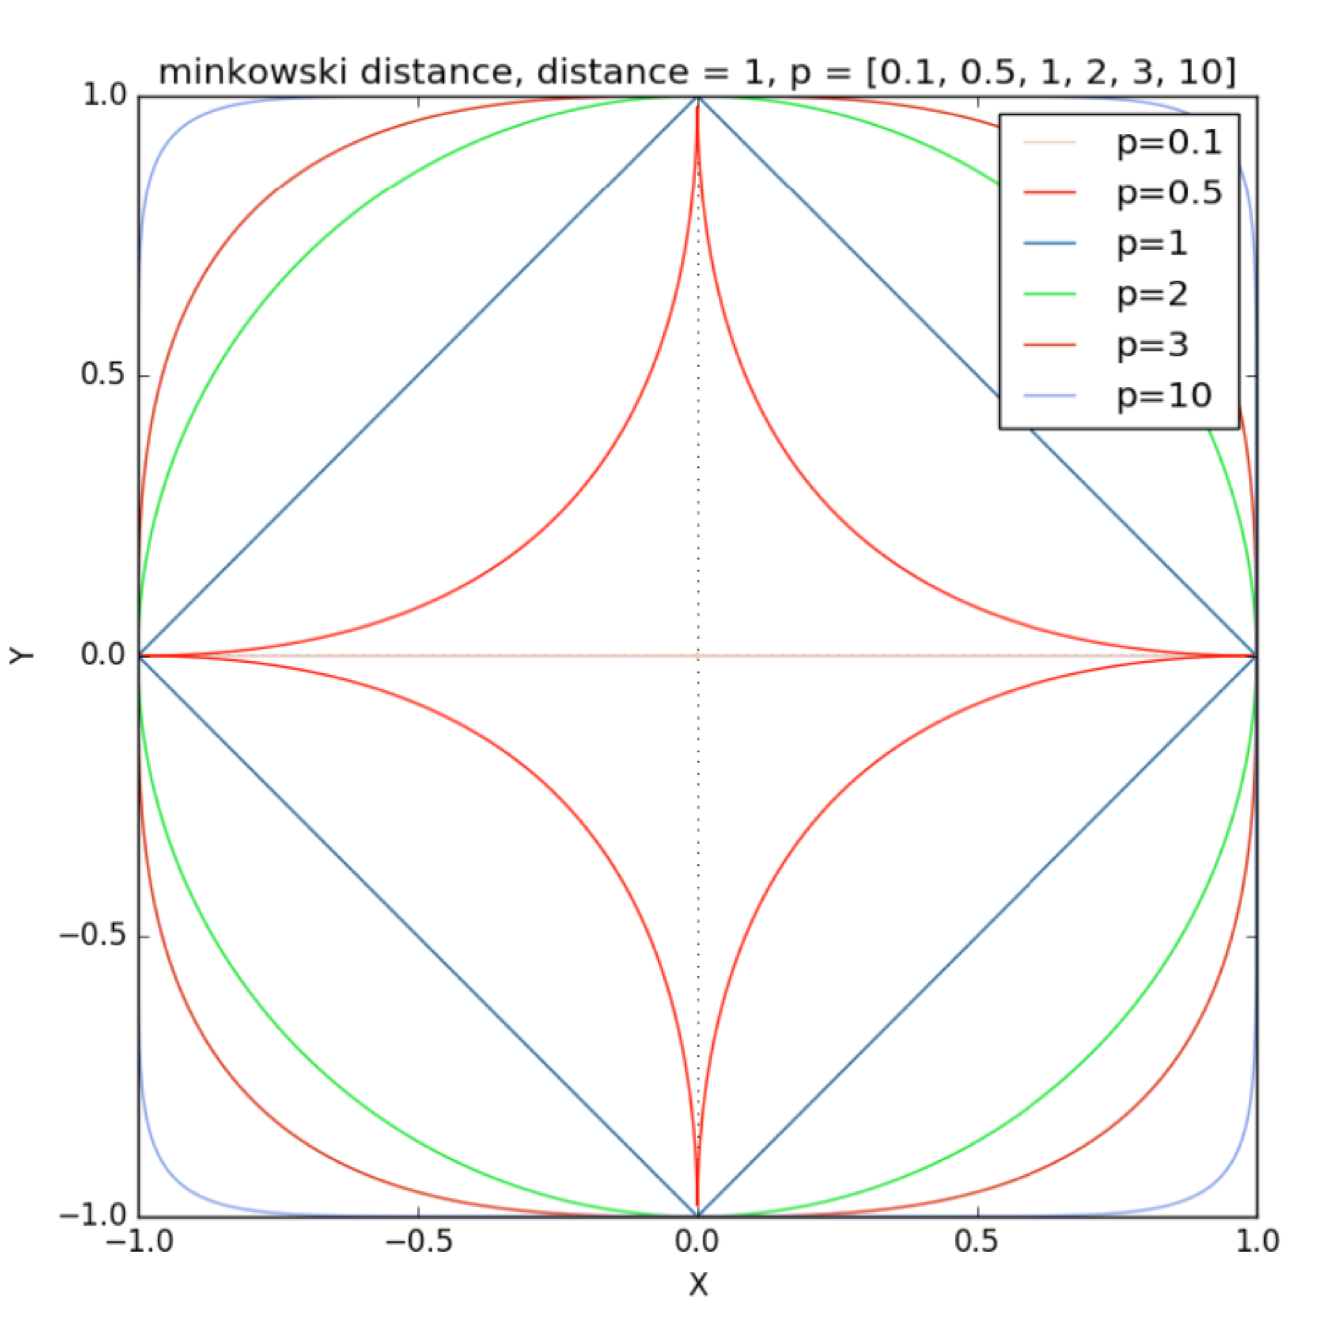
\includegraphics[width=0.5\linewidth]{figs/pnorm.png}
\end{figure}

为了证明 $p$-范数在 $p\geq 1$ 时满足三角不等式,首先需要证明一个引理和 Hölder 不等式。

\begin{lemma}
对任意实数 $\alpha>0,\beta>0$,都有 $\alpha\beta\leq \frac{\alpha^p}{p}+\frac{\beta^q}{q}$,其中 $p>1,q>1$ 且 $\frac{1}{p}+\frac{1}{q}=1$.
\end{lemma}
\begin{proof}
\begin{align*}
    \frac{\alpha^p}{p}+\frac{\beta^q}{q}&\geq\frac{q\alpha^p+p\beta^q}{pq}=\frac{q\alpha^p+p\beta^q}{p+q}\\
    &=\frac{(\alpha^p+\cdots+\alpha^p)+(\beta^q+\cdots+\beta^q)}{p+q}\\
    &\geq\sqrt[p+q]{\alpha^{pq}\beta^{pq}}=\sqrt[pq]{\alpha^{pq}\beta^{pq}}=\alpha\beta
\end{align*}
\end{proof}

\begin{theorem}[Hölder 不等式]
对任意 $\xi_k,\eta_k\in\mathbb C\,(k=1,\ldots,n)$,有:
\[
    \sum_{k=1}^n|\xi_k||\eta_k|\leq\left(\sum_{k=1}^n|\xi_k|^p\right)^{1/p}\left(\sum_{k=1}^n|\eta_k|^q\right)^{1/q}
\]
其中 $p>1,q>1$ 且 $\frac{1}{p}+\frac{1}{q}=1$.
\end{theorem}
\begin{proof}
令 $\alpha={|\xi_i|}/{\left(\sum_{k=1}^n|\xi_k|^p\right)^{1/p}}$,$\beta={|\eta_i|}/{\left(\sum_{k=1}^n|\eta_k|^q\right)^{1/q}}$,由引理得:
\[
    \frac{|\xi_i|}{\left(\sum_{k=1}^n|\xi_k|^p\right)^{1/p}}\cdot\frac{|\eta_i|}{\left(\sum_{k=1}^n|\eta_k|^q\right)^{1/q}}\leq\frac{|\xi_i|^p}{p\sum_{k=1}^n|\xi_k|^p}+\frac{|\eta_i|^q}{q\sum_{k=1}^n|\eta_k|^q}
\]
对 $i$ 求和:
\[
    \frac{\sum_{i=1}^n|\xi_i||\eta_i|}{\left(\sum_{k=1}^n|\xi_k|^p\right)^{1/p}\left(\sum_{k=1}^n|\eta_k|^q\right)^{1/q}}\leq\frac{1}{p}+\frac{1}{q}=1
\]
\end{proof}

接下来利用 Hölder 不等式就可以证明 $p$-范数满足三角不等式了。

\begin{proof}
设 $x,y\in\mathbb C^n$,当 $p\geq 1$ 时,有:
\begin{align*}
    \norm{x+y}_p^p&=\sum_{k=1}^n|x_k+y_k|^p\\
    &\leq\sum_{k=1}^n|x_k||x_k+y_k|^{p-1}+\sum_{k=1}^n|y_k||x_k+y_k|^{p-1}\\
    &\leq\left(\sum_{k=1}^n|x_k|^p\right)^{1/p}\left(\sum_{k=1}^n|x_k+y_k|^{q(p-1)}\right)^{1/q}\\&+\left(\sum_{k=1}^n|y_k|^p\right)^{1/p}\left(\sum_{k=1}^n|x_k+y_k|^{q(p-1)}\right)^{1/q}\\
    &=\left(\norm{x}_p+\norm{y}_p\right)\left(\sum_{k=1}^n|x_k+y_k|^{p}\right)^{1/q}\\
    &=\left(\norm{x}_p+\norm{y}_p\right)\norm{x+y}_p^{p/q}\\
    &=\left(\norm{x}_p+\norm{y}_p\right)\norm{x+y}_p^{p-1}
\end{align*}
于是:
\[
    \norm{x+y}_p\leq\left(\norm{x}_p+\norm{y}_p\right)
\]
\end{proof}

\begin{definition}[绝对范数,单调范数]
设 $x=(\xi_1,\ldots,\xi_n)^T\in\mathbb F^n$,记 $|x|=(|\xi_1|,\ldots,|\xi_n|)^T\in\mathbb R^n$,则称 $\mathbb F^n$ 上的范数 $v$ 为:
\begin{itemize}
    \item 绝对范数,若满足 $v(x)=v(|x|),\quad \forall x\in\mathbb F^n$;
    \item 单调范数,若满足 $|x|\leq |y|\implies v(x)\leq v(y),\quad \forall x,y\in\mathbb F^n$.
\end{itemize}
\end{definition}

\begin{theorem}
$\mathbb F^n$ 上的范数 $v$ 为绝对范数的充要条件是 $v$ 为单调范数。
\end{theorem}
\begin{proof}
充分性:设 $v$ 为单调范数,则对于任意 $x\in\mathbb F^n$,令 $y=|x|$,由于 $|x|\leq |y|$ 且 $|y|\geq|x|$,所以 $v(x)\leq v(y)$ 且 $v(y)\leq v(x)$,故 $v(x)=v(y)$,即 $v$ 为绝对范数。

必要性:设 $v$ 为绝对范数,则对于任意给定 $x\in\mathbb F^n$,任取 $k\in\{1,\ldots,n\}$,设 $\alpha\in[0,1]$,考察向量 $[x_1,\ldots,x_{k-1},\alpha x_k,x_{k+1},\ldots,x_n]^T$ 的范数,有:
\begin{align*}
    &v([x_1,\ldots,x_{k-1},\alpha x_k,x_{k+1},\ldots,x_n]^T)\\
    =\;&v\left(\frac{1-\alpha}{2}[x_1,\ldots,x_{k-1},-x_k,x_{k+1},\ldots,x_n]^T+\frac{1-\alpha}{2}x+\alpha x\right)\\
    \leq\;&\frac{1-\alpha}{2}v\left([x_1,\ldots,x_{k-1},-x_k,x_{k+1},\ldots,x_n]^T\right)+\frac{1-\alpha}{2}v(x)+\alpha v(x)\\
    =\;&\frac{1-\alpha}{2}v(x)+\frac{1-\alpha}{2}v(x)+\alpha v(x)=v(x)
\end{align*}
对各个分量反复应用上式,则对任意 $x\in\mathbb F^n$ 及任意 $\alpha_1,\ldots,\alpha_n\in[0,1]$,都有:
\[
    v([\alpha_1x_1,\ldots,\alpha_nx_n]^T)\leq v(x)
\]
最后,对 $\forall x,y\in\mathbb F^n$ 且 $\Vert x\Vert\leq\Vert y\Vert$,考虑每一个分量,存在 $\alpha_k\in[0,1]$ 和 $\theta_k$ 使得 $x_k=\alpha_ke^{i\theta_k}y_k$,因此:
\[
    v(x)=v([\alpha_1e^{i\theta_1}y_1,\ldots,\alpha_ne^{i\theta_n}y_n]^T)=v([\alpha_1|y_1|,\ldots,\alpha_n|y_n|]^T)\leq v(y)
\]
即 $v$ 是单调范数。
\end{proof}

\begin{definition}[对偶范数]
令 $\norm\cdot$ 为 $\mathbb R^n$ 上的范数,其对偶范数 $\norm\cdot^\ast$ 定义为:
\[
    \norm{z}^\ast=\sup_{\norm x\leq 1}\{z^Tx\}
\]
\end{definition}

\begin{property}
对偶范数的对偶是其本身,即 $\norm{x}^{\ast\ast}=\norm x$.
\end{property}

\begin{example}
$l_p$ 和 $l_q$ 互为对偶范数,其中 $\frac{1}{p}+\frac{1}{q}=1$.
\end{example}

\begin{definition}[范数等价]
对有限维空间 $V^n$ 中任意两个向量范数 $\norm x_\alpha,\norm x_\beta$,若存在正常数 $c_1,c_2$,使得:
\[
    c_1\norm{x}_\beta\leq\norm{x}_\alpha\leq c_2\norm{x}_\beta,\quad\forall x\in V^n
\]
则称范数 $\norm{x}_\alpha$ 与 $\norm{x}_\beta$ 等价。
\end{definition}
\begin{com}
范数等价是一个\textbf{等价关系},即满足\textbf{自反性、对称性、传递性}。
\end{com}

\begin{theorem}
有限维空间中任意两个向量范数都等价。
\end{theorem}
\begin{proof}
由于等价关系具有传递性,我们只需要证明任意一个向量范数都等价于 2-范数即可。
令 $f(x)=\norm{x}$ 为 $V^n$ 上的任一向量范数,由于当 $x\to y$ 时,$\left|\norm x-\norm y\right|\leq \norm{x-y}\to 0$,因此范数是连续函数。于是 $f(x)$ 在单位超球面上有大于零的最小值和最大值:
\[
    0<\min_{\norm{x}_2=1}f(x)\leq \max_{\norm{x}_2=1}f(x)
\]
记上述最小值为 $c_1$,最大值为 $c_2$,于是:
\[
    c_1\leq \left\Vert\frac{x}{\norm{x}_2}\right\Vert\leq c_2\implies c_1\norm{x}_2\leq\norm{x}\leq c_2\norm{x}_2
\]
故 $\norm\cdot$ 与 2-范数等价。
\end{proof}

\begin{definition}[依范数收敛]
设 $\{x^{(k)}\}$ 是 $V^n$ 中的向量序列,若存在 $x\in V^n$,使得:
\[
    \lim_{k\to\infty} \norm{x^{(k)}-x}_\alpha=0
\]
则称序列 $\{x^{(k)}\}$ 依 $\alpha$ 范数收敛到 $x$.
\end{definition}

\begin{theorem}
向量序列各分量收敛等价于依范数收敛,即:
\[
    \lim_{k\to\infty} x^{(k)}=x\iff\lim_{k\to\infty} \norm{x^{(k)}-x}=0
\]
\end{theorem}
\begin{proof}
由于向量范数的等价性,只需要对 1-范数证明即可。
\begin{align*}
    x^{(k)}\to x&\iff \xi_i^{(k)}\to\xi_i,\quad i=1,\ldots,n\\
    &\iff |\xi_i^{(k)}-\xi_i|\to 0,\quad i=1,\ldots,n\\
    &\iff \sum_{i=1}^n|\xi_i^{(k)}-\xi_i|\to 0\\
    &\iff \norm{x^{(k)}-x}_1\to0
\end{align*}
\end{proof}

\subsection{矩阵范数}

\begin{definition}[广义矩阵范数]
与向量范数相同,满足 3 条性质:
\begin{enumerate}[series=matrix-norm]
    \item 非负性:$\norm{A}\geq 0$ 且 $\norm{A}=0\iff A=0$
    \item 齐次性:$\norm{kA}=|k|\norm{A},\,k\in K$
    \item 三角不等式:$\norm{A+B}\leq\norm{A}+\norm{B}$
\end{enumerate}
\end{definition}

\begin{definition}[矩阵范数]
在广义矩阵范数的基础上增加相容条件:
\begin{enumerate}[resume=matrix-norm]
    \item 相容性:$\norm{AB}\leq\norm{A}\norm{B}$
\end{enumerate}
\end{definition}

\begin{remark}
对于涉及到矩阵范数的不等式放缩,一般就是考虑三角不等式和相容性。
\end{remark}

\begin{definition}[相容范数]
对 $\mathbb C^{m\times n}$ 上的矩阵范数 $\norm{A}_M$ 和 $\mathbb C^m,\mathbb C^n$ 上的同类向量范数 $\norm{x}_v$,若:
\[
    \norm{Ax}_v\leq \norm{A}_M\norm{x}_v,\quad \forall A\in\mathbb C^{m\times n},\,\forall x\in\mathbb C^n
\]
则称矩阵范数 $\norm{A}_M$ 与向量范数 $\norm{x}_v$ 是相容的。
\end{definition}

\begin{remark}
简单地说,把矩阵视作线性映射,则相容范数表示,映射后的向量与原向量的长度的相对变化量被矩阵范数所控制。
\end{remark}

\begin{example}[$m_1$ 范数]
设 $A\in\mathbb C^{m\times n}$,矩阵的 $m_1$ 范数与向量的 1-范数定义类似:
\[
    \norm{A}_{m_1}=\sum_{i=1}^m\sum_{j=1}^n|a_{ij}|
\]
即所有元素的绝对值(模)之和。可以证明 \textbf{$m_1$ 范数是矩阵范数,并且与向量的 1-范数相容}。
\end{example}

\begin{proof}
非负性、齐次性和三角不等式与向量的 1-范数完全相同,必然成立,只需证明矩阵范数的相容性以及与向量 1-范数的相容性。

相容性:
\begin{align*}
    \norm{AB}_{m_1}&=\sum_{i=1}^m\sum_{j=1}^l\left|\sum_{k=1}^na_{ik}b_{kj}\right|\\
    &\leq\sum_{i=1}^m\sum_{j=1}^l\sum_{k=1}^n|a_{ik}||b_{kj}|\\
    &\leq\sum_{k=1}^n\left[\left(\sum_{i=1}^m|a_{ik}|\right)\left(\sum_{j=1}^l|b_{kj}|\right)\right]\\
    &\leq\left(\sum_{k=1}^n\sum_{i=1}^m|a_{ik}|\right)\left(\sum_{k=1}^n\sum_{j=1}^l|b_{kj}|\right)\\
    &=\norm{A}_{m_1}\norm{B}_{m_1}
\end{align*}

与向量的 1-范数相容:
\begin{align*}
    \norm{Ax}_1&=\sum_{i=1}^m\left|\sum_{j=1}^na_{ij}x_j\right|\\
    &\leq\sum_{i=1}^m\sum_{j=1}^n|a_{ij}||x_j|\\
    &\leq\left(\sum_{i=1}^m\sum_{j=1}^n|a_{ij}|\right)\left(\sum_{j=1}^n|x_j|\right)\\
    &=\norm{A}_{m_1}\norm{x}_1
\end{align*}    
\end{proof}

\begin{definition}[$m_\infty$ 范数]
设 $A\in\mathbb C^{m\times n}$,矩阵的 $m_\infty$ 范数与向量的无穷范数定义类似,\textbf{但是要乘以 $n$},否则不满足相容性:
\[
    \norm{A}_{m_\infty}=n\cdot\max_{i,j}|a_{ij}|
\]
可以证明 \textbf{$m_\infty$ 范数是矩阵范数,且与向量的无穷范数相容}。
\end{definition}
\begin{proof}
相容性:
\begin{align*}
\norm{AB}_{m_\infty}&=n\cdot\max_{i,j}\left|\sum_{k=1}^n a_{ik}b_{kj}\right|\\
&\leq n\cdot\max_{i,j}\sum_{k=1}^n |a_{ik}||b_{kj}|\\
&\leq n\cdot\max_{i,j}\left[n\cdot(\max_k |a_{ik}|)(\max_k |b_{kj}|)\right]\\
&=\max_{i,j}\left[(n\cdot \max_k |a_{ik}|)(n\cdot\max_k |b_{kj}|)\right]\\
&=(n\cdot \max_{i,k} |a_{ik}|)(n\cdot\max_{k,j} |b_{kj}|)\\
&=\norm{A}_{m_\infty}\norm{B}_{m_\infty}
\end{align*}

与向量的无穷范数相容:
\begin{align*}
\norm{Ax}_{\infty}&=\max_i\left|\sum_{j=1}^na_{ij}x_j\right|\\
&\leq\max_i\sum_{j=1}^n|a_{ij}||x_j|\\
&\leq\max_i\left[n\cdot(\max_j |a_{ij}|)(\max_j |x_j|)\right]\\
&=n\cdot\max_{i,j}|a_{ij}|\cdot\max_j |x_j|\\
&=\norm{A}_{m_\infty}\norm{x}_{\infty}
\end{align*}
\end{proof}

\begin{definition}[Frobenius 范数]
设 $A\in\mathbb C^{m\times n}$,矩阵的 F-范数与向量的 2-范数定义类似:
\[
    \norm{A}_{F}=\norm{A}_{m_2}=\left(\sum_{i=1}^m\sum_{j=1}^n|a_{ij}|^2\right)^{1/2}=\left(\text{tr}(A^HA)\right)^{1/2}
\]
可以证明 \textbf{F-范数是矩阵范数,并且与向量的 2-范数相容}。
\end{definition}
\begin{proof}
相容性:
\begin{align*}
\norm{AB}_F^2&=\sum_{i=1}^m\sum_{j=1}^l\left|\sum_{k=1}^na_{ik}b_{kj}\right|^2\\
&\leq\sum_{i=1}^m\sum_{j=1}^l\left(\sum_{k=1}^n|a_{ik}||b_{kj}|\right)^2\\
&\leq\sum_{i=1}^m\sum_{j=1}^l\left(\sum_{k=1}^n|a_{ik}|\right)^2\left(\sum_{k=1}^n|b_{kj}|\right)^2\\
&\leq\left(\sum_{i=1}^m\sum_{k=1}^n|a_{ik}|\right)^2\left(\sum_{j=1}^l\sum_{k=1}^n|b_{kj}|\right)^2\\
&=\norm{A}_F^2\norm{B}_F^2
\end{align*}

与向量的 2-范数相容:
\begin{align*}
\norm{Ax}_2^2&=\sum_{i=1}^m\left|\sum_{j=1}^n a_{ij}x_j\right|^2\\
&\leq\sum_{i=1}^m\left(\sum_{j=1}^n |a_{ij}||x_j|\right)^2\\
&\leq\sum_{i=1}^m\left(\sum_{j=1}^n |a_{ij}|\right)^2\left(\sum_{j=1}^n|x_j|\right)^2\\
&\leq\left(\sum_{i=1}^m\sum_{j=1}^n |a_{ij}|\right)^2\left(\sum_{j=1}^n|x_j|\right)^2\\
&=\norm{A}_F^2\norm{x}_2^2
\end{align*}
\end{proof}

\begin{theorem}[Frobenius 范数的酉不变性]
设 $A\in\mathbb C^{m\times n}$,酉矩阵 $P\in\mathbb C^{m\times n},\,Q\in\mathbb C^{n\times n}$,则:
\[
    \norm{PA}_F=\norm{A}_F=\norm{AQ}_F
\]
\end{theorem}
\begin{proof}
\begin{align*}
    &\norm{PA}_F^2=\text{tr}\left((PA)^H(PA)\right)=\text{tr}\left(A^HP^HPA\right)=\text{tr}\left(A^HA\right)=\norm{A}_F^2\\
    &\norm{AQ}_F^2=\text{tr}\left((AQ)^H(AQ)\right)=\text{tr}\left(Q^HA^HAQ\right)=\text{tr}\left(A^HAQQ^H\right)=\text{tr}\left(A^HA\right)=\norm{A}_F^2
\end{align*}
\begin{com}
证明过程用到了结论 \ref{cor:trace}:$\text{tr}(ABC)=\text{tr}(BCA)$.
\end{com}
\end{proof}

\begin{corollary}
矩阵的 F-范数等于所有奇异值平方和开根,即:
\[
    \norm{A}_F=\left(\sigma_1^2+\cdots+\sigma_r^2\right)^{1/2}
\]
\end{corollary}
\begin{proof}
根据奇异值分解和酉不变性易证。
\end{proof}

\begin{property}
转置和共轭都不改变矩阵的 F-范数,即:
\[
    \norm{A}_F=\norm{A^T}_F=\norm{\bar A}_F=\norm{A^H}_F
\]
\end{property}

\begin{theorem}
对于 $\mathbb C^{m\times n}$ 上的矩阵范数 $\norm{A}$,存在向量范数 $\norm{x}_v$,使得 $\norm{Ax}_v\leq\norm{A}\norm{x}_v$.
\end{theorem}
\begin{proof}
任取非零向量 $y\in\mathbb C^n$,则按如下方式构造向量范数即可:
\[
    \norm{x}_v=\norm{xy^H}
\]
首先由于它是由矩阵范数定义的,所以必然满足向量范数的 3 条性质,即确实是一个向量范数。其次证明相容性:
\[
    \norm{Ax}_v=\norm{Axy^H}\leq\norm{A}\norm{xy^H}=\norm{A}\norm{x}_v
\]
\end{proof}

\begin{definition}[从属范数]
已知 $\mathbb C^m$ 和 $\mathbb C^n$ 上的同类向量范数 $\norm{x}_v$,设 $A\in\mathbb C^{m\times n}$,定义函数:
\[
    \norm{A}=\max_{\norm{x}_v=1}\norm{Ax}_v=\max_{x\neq 0}\frac{\norm{Ax}_v}{\norm{x}_v}
\]
则 $\norm{A}$ 是矩阵范数,且与 $\norm{x}_v$ 相容。
\end{definition}
\begin{proof}
只需依次证明非负性、齐次性、三角不等式、与向量范数相容和矩阵范数的相容性即可。
\begin{enumerate}
    \item 非负性:若 $A\neq0$,则存在 $x_0$ 满足 $\norm{x_0}_v=1$ 且 $Ax_0\neq 0$,于是:
    \[\norm{A}\geq\norm{Ax_0}_v>0\]
    若 $A=0$,则:
    \[\norm{A}=\max_{\norm{x}_v=1}\norm{Ax}_v=\max_{\norm{x}_v=1}\norm{0}_v=0\]

    \item 齐次性:
    \[
        \norm{kA}=\max_{\norm{x}_v=1}\norm{kAx}_v=k\cdot\max_{\norm{x}_v=1}\norm{Ax}_v=k\norm{A}
    \]

    \item 三角不等式:
    \begin{align*}
        \norm{A+B}&=\max_{\norm{x}_v=1}\norm{(A+B)x}_v
        \leq\max_{\norm{x}_v=1}(\norm{Ax}_v+\norm{Bx}_v)\\
        &\leq\max_{\norm{x}_v=1}\norm{Ax}_v+\max_{\norm{x}_v=1}\norm{Bx}_v
        =\norm{A}+\norm{B}\\
    \end{align*}

    \item 与 $\norm{x}_v$ 的相容:若 $x=0$ 显然成立;若 $x\neq 0$,设 $x_0=x/\norm{x}_v$,则:
    \[
        \norm{Ax_0}_v\leq\max_{\norm{x}_v=1}\norm{Ax}_v=\norm{A}
    \]
    故:
    \[
        \norm{Ax}_v=\big\Vert{A(\norm{x}_v\cdot x_0)}\big\Vert=\norm{Ax_0}\norm{x}_v\leq\norm{A}\norm{x}_v
    \]

    \item 相容性:
    \[
        \norm{AB}=\max_{\norm{x}_v=1}\norm{ABx}_v=\norm{A(Bx^\ast)}_v\leq\norm{A}\norm{Bx^\ast}_v\leq\norm{A}\norm{B}
    \]
    其中,$x^\ast$ 是使得 $\norm{ABx}_v$ 取到最大值的单位向量。

\end{enumerate}
\end{proof}

\begin{property}
从属范数一定有 $\norm{I}=1$,但一般的矩阵范数并不一定 ,例如  $\norm{I}_{m_1}=n,\,\norm{I}_F=\sqrt{n}$.
\end{property}

\begin{example}[1-范数/列范数]
由向量的 1-范数诱导出的矩阵范数:
\[
    \norm{A}_1=\max_{j}\sum_{i=1}^m|a_{ij}|
\]
即对各列的元素求绝对值(模)的和,选最大的和。
\end{example}
\begin{proof}
记 $t=\max_{j}\sum_{i=1}^m|a_{ij}|$,我们只需要证明 $\norm{A}_1\leq t$ 且 $\norm{A}_1\geq t$ 即可。

首先,设 $x\in\mathbb C^n$ 且 $\norm{x}_1=1$,则:
\begin{align*}
    \norm{Ax}_1&=\sum_{i=1}^m\left|\sum_{j=1}^na_{ij}x_j\right|\\
    &\leq\sum_{i=1}^m\sum_{j=1}^n|a_{ij}||x_j|\\
    &=\sum_{j=1}^n\left(|x_j|\cdot\sum_{i=1}^m|a_{ij}|\right)\\
    &\leq\sum_{j=1}^n\left(|x_j|\cdot t\right)
    =t\cdot\norm{x}_1=t
\end{align*}
由于上式对任意长度为 1 的 $x$ 都成立,因此 $\norm{A}_1\leq t$.

其次,设 $k=\mathop{\text{argmax }}_{j}\sum_{i=1}^m|a_{ij}|$,即 $t=\sum_{i=1}^m|a_{ik}|$;再设 $e_k=(0,\ldots,1,\ldots,0)^T$,则:
\[
    \norm{A}_1\geq\norm{Ae_k}_1=\sum_{i=1}^m|a_{ik}|=t
\]
综上,$\norm{A}_1=t$.
\end{proof}

\begin{example}[无穷范数/行范数]
由向量的无穷范数诱导出的矩阵范数:
\[
    \norm{A}_\infty=\max_i\sum_{j=1}^n|a_{ij}|
\]
即对各行的元素求绝对值(模)的和,选最大的和。
\end{example}
\begin{proof}
记 $t=\max_{i}\sum_{j=1}^n|a_{ij}|$,我们只需要证明 $\norm{A}_\infty\leq t$ 且 $\norm{A}_\infty\geq t$ 即可。

首先,设 $x\in\mathbb C^n$ 且 $\norm{x}_\infty=1$,则 $|x_j|\leq 1$,于是:
\begin{align*}
    \norm{Ax}_\infty&=\max_{i=1}^m\left|\sum_{j=1}^na_{ij}x_j\right|\\
    &\leq\max_{i=1}^m\sum_{j=1}^n|a_{ij}||x_j|\\
    &\leq\max_{i=1}^m\sum_{j=1}^n|a_{ij}|=t
\end{align*}
由于上式对任意长度为 1 的 $x$ 都成立,因此 $\norm{A}_\infty\leq t$.

其次,设 $\mathbf1=(1,\ldots,1)^T$,则:
\[
    \norm{A}_\infty\geq\norm{A\mathbf1}_\infty=\max_{i=1}^m\sum_{j=1}^n|a_{ij}|=t
\]
综上 $\norm{A}_\infty=t$.
\end{proof}

\begin{example}[2-范数/谱范数]
由向量的 2-范数诱导出的矩阵范数:
\[
    \norm{A}_2=\max_j\sqrt{\lambda_j(A^HA)}=\sigma_1
\]
即 $A$ 的最大奇异值。
\end{example}
\begin{proof}
设 $A$ 的奇异值分解为 $A=U\Sigma V^H$,其中 $U,V$ 都是酉矩阵。则:
\begin{align*}
    \norm{A}_2&=\max_{x\neq 0}\frac{\norm{Ax}_2}{\norm{x}_2}
    =\max_{x\neq 0}\frac{\norm{U\Sigma V^Hx}_2}{\norm{x}_2}
    =\max_{x\neq 0}\frac{\norm{\Sigma V^Hx}_2}{\norm{V^Hx}_2}\\
    &=\max_{y\neq 0}\frac{\norm{\Sigma y}_2}{\norm{y}_2}
    =\max_{\norm{y}_2=1}\norm{\Sigma y}_2=\max_{\norm{y}_2=1}\left(\sum_{i=1}^ny_i^2\sigma_i^2\right)^{1/2}
\end{align*}
显然当 $y=(1,0,\ldots,0)^T$ 时上式取到最大值 $\sigma_1$.
\end{proof}

\begin{theorem}[谱范数的酉不变性]
设 $A\in\mathbb C^{m\times n}$,酉矩阵 $P\in\mathbb C^{m\times n},\,Q\in\mathbb C^{n\times n}$,则:
\[
    \norm{PA}_2=\norm{A}_2=\norm{AQ}_2
\]
\end{theorem}
\begin{proof}
由于酉变换不改变矩阵的奇异值,因此谱范数是酉不变范数。
\end{proof}

\subsection{范数的一些应用}

\begin{theorem}
设有 $\mathbb C^{n\times n}$ 上的矩阵范数 $\norm\cdot$,若矩阵 $A\in\mathbb C^{n\times n}$ 满足:
\[\norm{A}<1\]
则 $I-A$ 非奇异,且:
\begin{align*}
    &\norm{(I-A)^{-1}}\leq\frac{\norm{I}}{1-\norm{A}}\\
    &\norm{I-(I-A)^{-1}}\leq\frac{\norm{A}}{1-\norm{A}}
\end{align*}
\end{theorem}
\begin{proof}
(1). 证明 $I-A$ 非奇异:选取与 $\norm{A}$ 相容的向量范数 $\norm{x}_v$(根据前文的定理,一定存在这样的向量范数)。假设 $\det(I-A)=0$,则取 $x_0\in N(I-A)$,有:
\[
    (I-A)x_0=0\implies x_0=Ax_0\implies\norm{x_0}_v=\norm{Ax_0}_v\leq\norm{A}\norm{x_0}_v<\norm{x_0}_v
\]
因此假设不成立,故 $I-A$ 非奇异。

(2). 证明第一个不等式:
\begin{align*}
    (I-A)^{-1}(I-A)=I&\implies(I-A)^{-1}=I+(I-A)^{-1}A\\
    &\implies\norm{(I-A)^{-1}}\leq\norm{I}+\norm{(I-A)^{-1}A}\\
    &\implies\norm{(I-A)^{-1}}\leq\norm{I}+\norm{(I-A)^{-1}}\norm{A}\\
    &\implies\norm{(I-A)^{-1}}\leq\frac{\norm{I}}{1-\norm{A}}\\
\end{align*}

(3). 证明第二个不等式:
\begin{align*}
    (I-A)-I=-A&\implies I-(I-A)^{-1}=-A(I-A)^{-1}\\
    &\implies A-A(I-A)^{-1}=-A^2(I-A)^{-1}\\
    &\implies A(I-A)^{-1}=A+A^2(I-A)^{-1}\\
    &\implies\norm{A(I-A)^{-1}}\leq\norm{A}+\norm{A}\norm{A(I-A)^{-1}}\\
    &\implies\norm{A(I-A)^{-1}}\leq\frac{\norm{A}}{1-\norm{A}}\\
    &\implies\norm{I-(I-A)^{-1}}=\norm{-A(I-A)^{-1}}\leq\frac{\norm{A}}{1-\norm{A}}
\end{align*}
\begin{com}
(2)、(3) 的证明思路可以从后往前推。
\end{com}
\end{proof}

\begin{definition}[条件数]
设 $A\in\mathbb C^{n\times n}$ 可逆,其条件数定义为:
\[
    \text{cond}(A)=\norm{A}\norm{A^{-1}}
\]
\end{definition}

\paragraph{线性方程组扰动分析}
条件数反映了 $A^{-1}$ 对扰动的敏感程度。例如,设有线性方程组 $Ax=b$,其扰动解满足:
\[
    (A+\delta A)(x+\delta x)=b+\delta b
\]
那么:
\[
    Ax+\delta A\cdot x+A\cdot \delta x+\delta A\cdot \delta x=b+\delta b\implies \delta A\cdot x+A\cdot \delta x\approx\delta b
\]
故:
\[
    \delta x=A^{-1}\delta b-A^{-1}\delta A\cdot x
\]
两边取范数并放大:
\begin{align*}
    \norm{\delta x}&=\norm{A^{-1}\delta b-A^{-1}\delta A\cdot x}\\
    &\leq\norm{A^{-1}\delta b}+\norm{A^{-1}\delta A\cdot x}\\
    &\leq\norm{A^{-1}}\norm{\delta b}+\norm{A^{-1}}\norm{\delta A}\norm{x}
\end{align*}
再根据 $\norm{A}\norm{x}\geq\norm{b}$,于是:
\begin{align*}
    \frac{\norm{\delta x}}{\norm{x}}&\leq\frac{\norm{A^{-1}}\norm{\delta b}}{\norm{x}}+\norm{A^{-1}}\norm{\delta A}\\
    &\leq\norm{A}\norm{A^{-1}}\frac{\norm{\delta b}}{\norm{b}}+\norm{A}\norm{A^{-1}}\frac{\norm{\delta A}}{\norm{A}}\\
    &=\text{cond}(A)\left(\frac{\norm{\delta b}}{\norm{b}}+\frac{\norm{\delta A}}{\norm{A}}\right)
\end{align*}
也就是说,解的相对扰动被输入 $A,b$ 的相对扰动和条件数控制。如果 $A$ 的条件数很大,那么解的误差就会很大。

\paragraph{谱半径及其性质}

\begin{definition}[谱半径]
设 $A\in\mathbb C^{n\times n}$ 的特征值为 $\lambda_1,\ldots,\lambda_n$,则谱半径定义为:
\[
    \rho(A)=\max_i|\lambda_i|
\]
\end{definition}
\begin{theorem}[谱半径是矩阵范数的下确界]
\label{thm:specrad-norm}
设 $A\in\mathbb C^{n\times n}$,则对任意一种矩阵范数都有:
\[
    \rho(A)\leq\norm{A}
\]
而对任意 $\epsilon>0$,必然存在某种矩阵范数,使得:
\[
    \norm{A}\leq \rho(A)+\epsilon
\]
\end{theorem}
\begin{proof}
首先证明第一个关系式。设 $\lambda$ 为 $A$ 的特征值,$x$ 为对应特征向量,$\norm{\cdot}_v$ 为与 $\norm{A}$ 相容的向量范数,则:
\[
    |\lambda|\norm{x}_v=\norm{\lambda x}_v=\norm{Ax}_v\leq\norm{A}\norm{x}_v\implies |\lambda|\leq\norm{A}
\]
于是:
\[
    \rho(A)=\max_i|\lambda_i|\leq\norm{A}
\]

然后证明第二个关系式。将 $A$ 相似变换为 Jordan 标准形,即存在 $P\in\mathbb C^{n\times n}$,使得:
\[
    P^{-1}AP=\Lambda+\tilde I=\text{diag}(\lambda_1,\ldots,\lambda_n)+
    \begin{bmatrix}
    0&\delta_1&&&\\
    &0&\delta_2&&\\
    &&\ddots&\ddots&\\
    &&&0&\delta_{n-1}\\
    &&&&0
    \end{bmatrix}
\]
其中 $\delta_i$ 为 0 或 1.  构造对角矩阵 $D=\text{diag}(1,\epsilon,\ldots,\epsilon^{n-1})$,设 $S=PD$,则:
\[
    S^{-1}AS=D^{-1}P^{-1}APD=D^{-1}(\Lambda+\tilde I)D=\Lambda+D^{-1}\tilde ID=\Lambda+\epsilon\tilde I
\]
于是:
\[
    \norm{S^{-1}AS}_1\leq\norm{\Lambda}_1+\epsilon\norm{\tilde I}_1\leq\rho(A)+\epsilon
\]
因此,构造矩阵范数:
\[
    \norm{A}_M=\norm{S^{-1}AS}_1
\]
即可满足 $\norm{A}_M\leq\rho(A)+\epsilon$.
\end{proof}

\begin{note}
上述证明过程中构造的范数与矩阵 $A$ 有关,\textbf{实际上不存在这样的矩阵范数对任意矩阵都成立}。
\end{note}

\begin{remark}
上述关系也可以表述为:
\[
    \rho(A)=\inf_\alpha\norm{A}_\alpha
\]

可视化如下:

\begin{figure}[H]
    \centering
    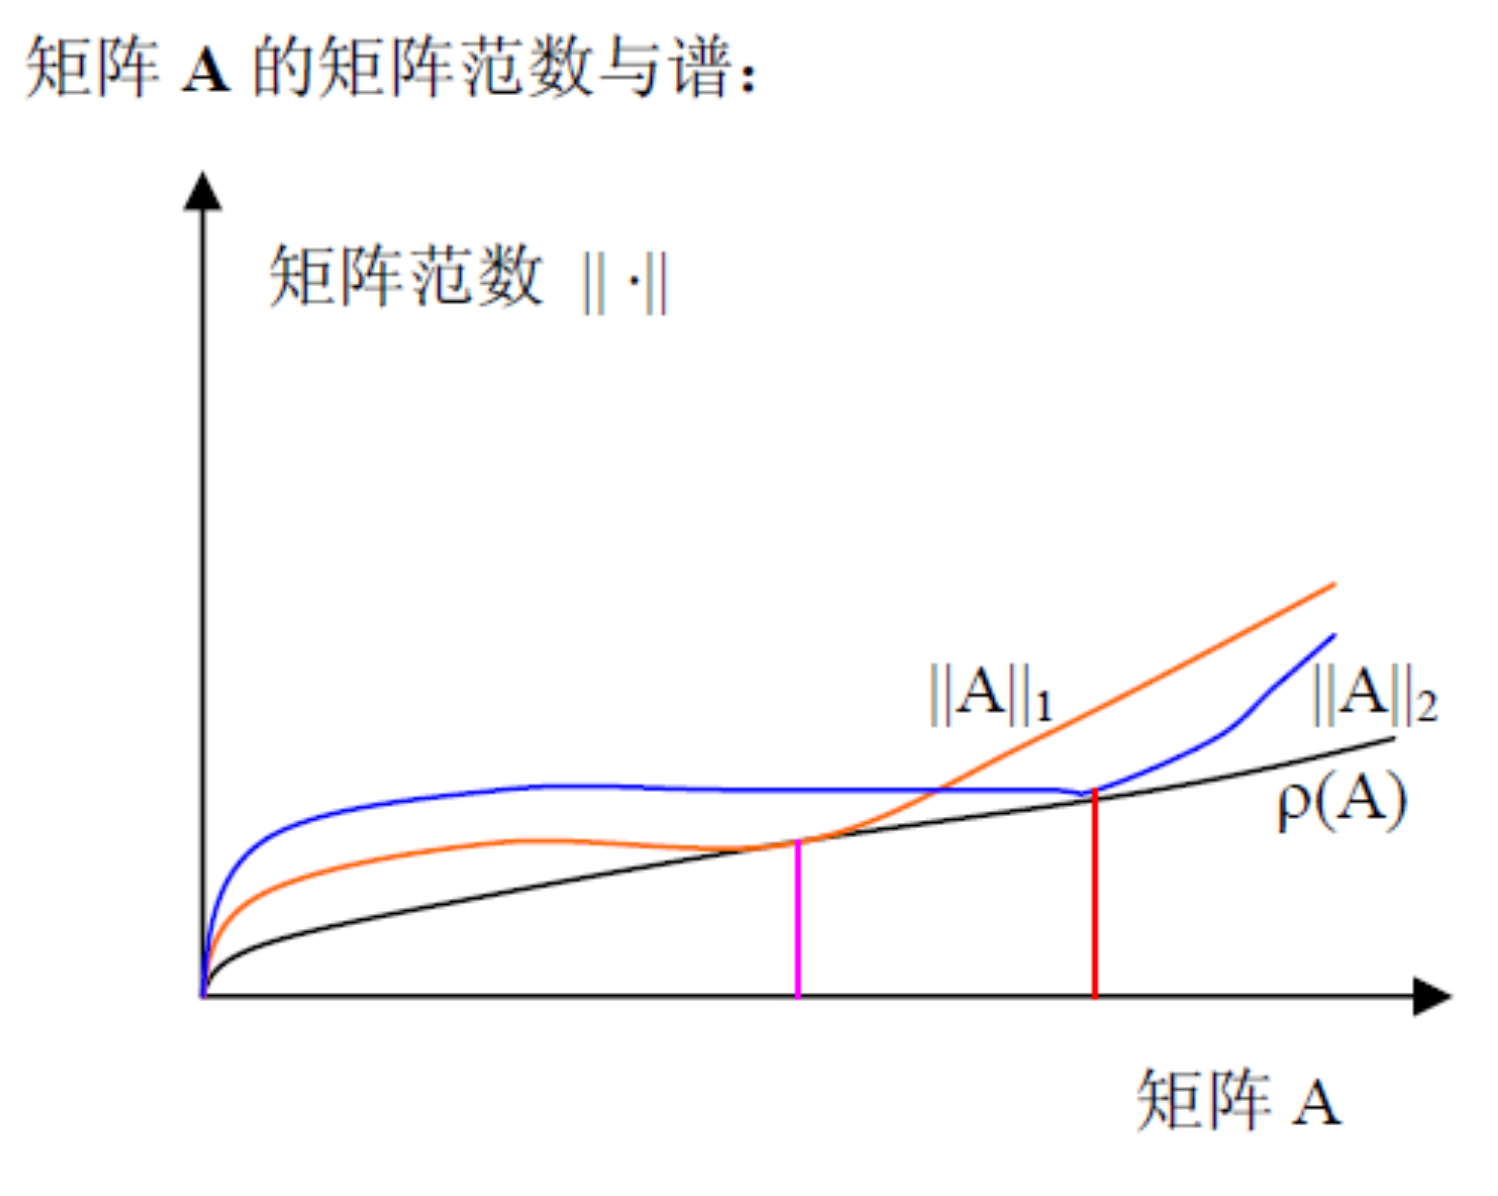
\includegraphics[width=0.4\linewidth]{figs/rho.png}
\end{figure}
\end{remark}
